\section{Исследование}

\begin{figure}[ht]
	\centering
	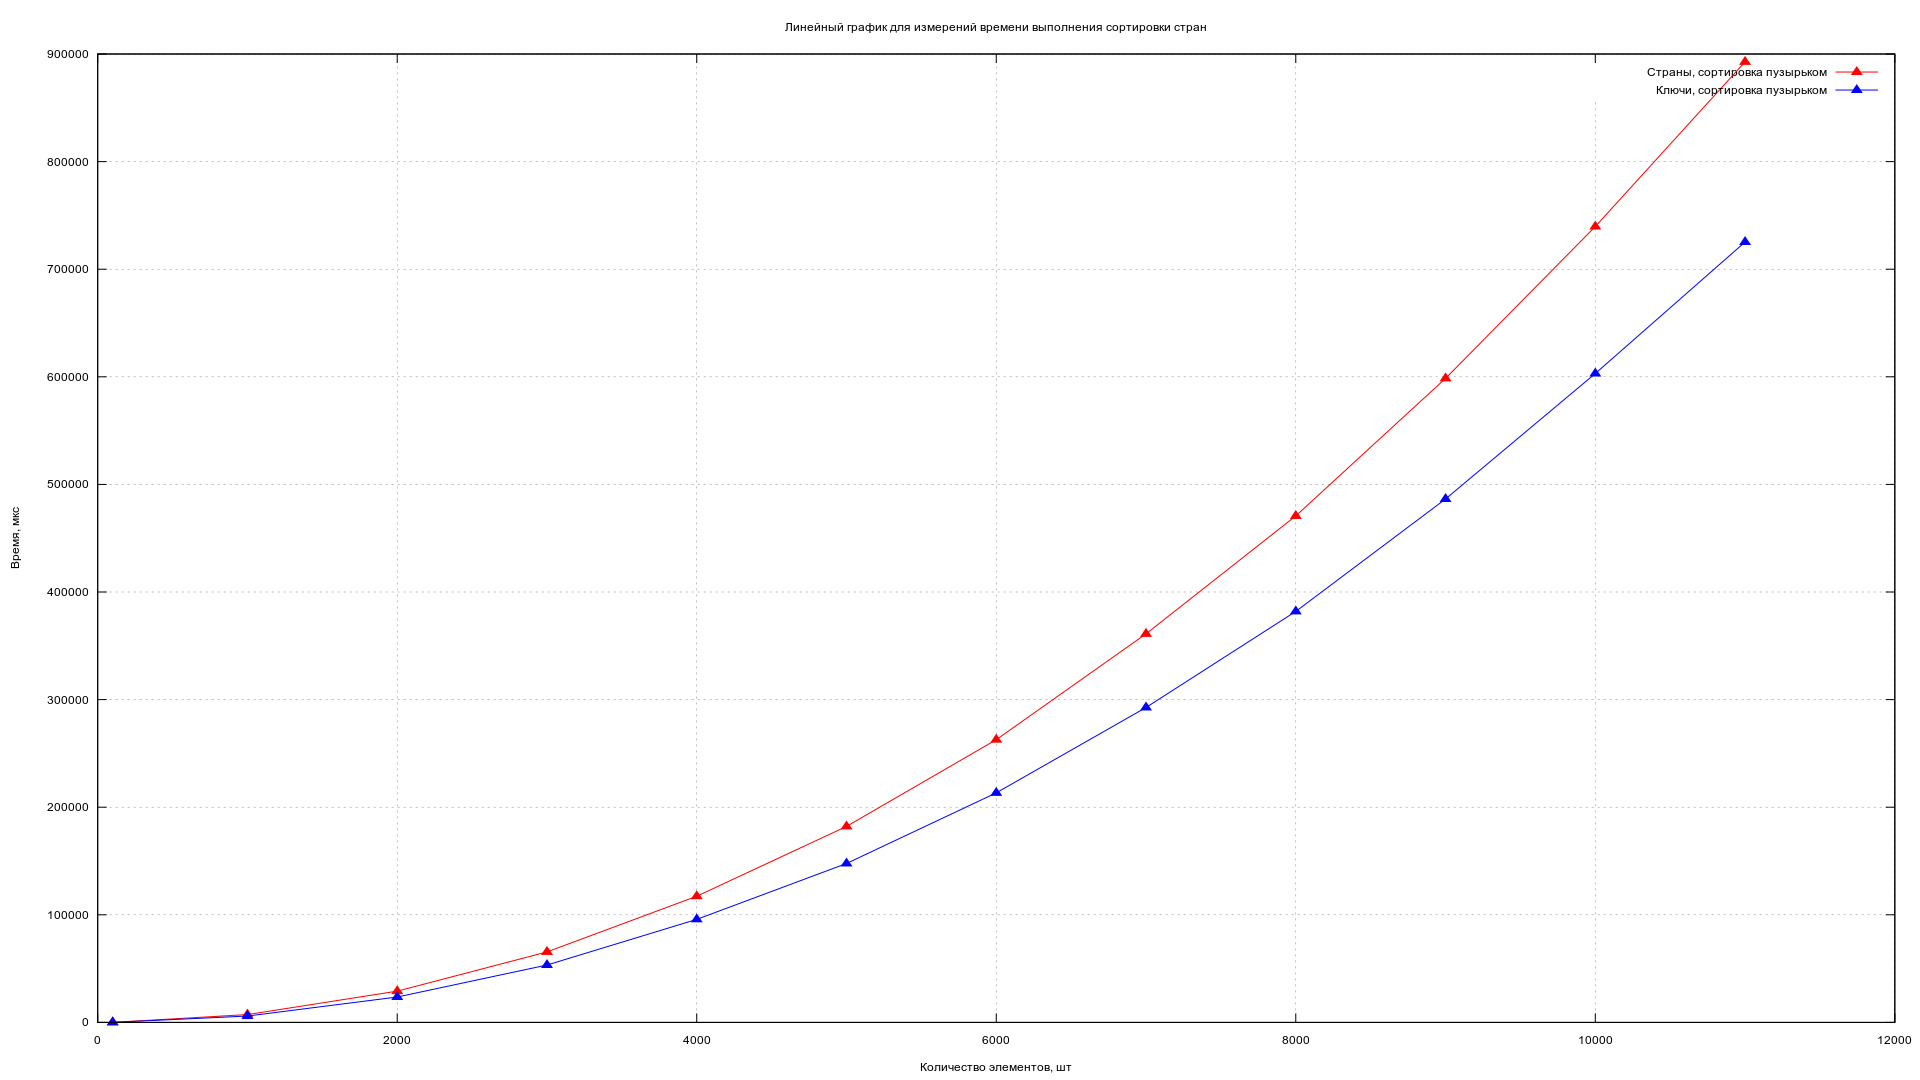
\includegraphics[width=0.9\textwidth]{img/linear_time_buble.jpg}
	\captionsetup{font=footnotesize}
	\caption{Зависимость времени между сортировкой стран и ключей}
	\label{fig:01}
\end{figure}

\begin{figure}[ht]
	\centering
	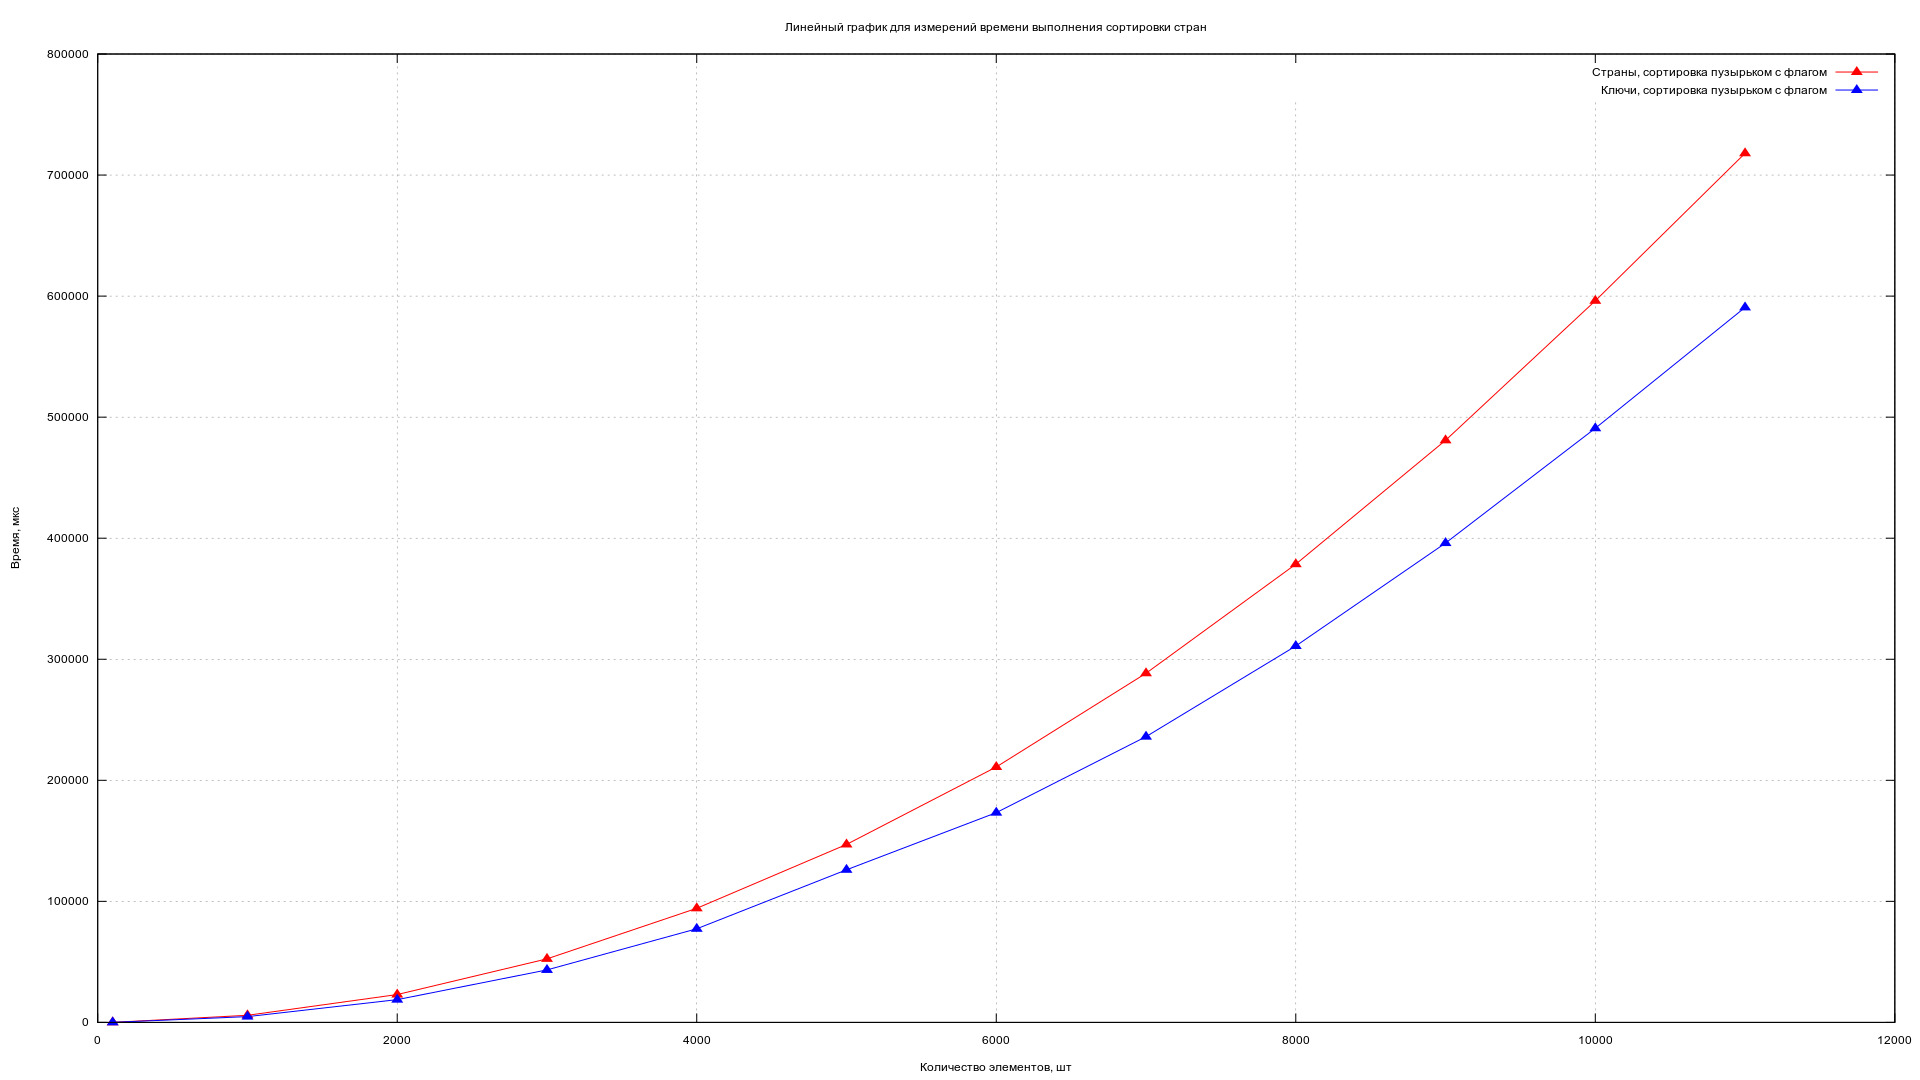
\includegraphics[width=0.9\textwidth]{img/linear_time_flag_buble.jpg}
	\captionsetup{font=footnotesize}
	\caption{Зависимость времени между сортировкой с флагом стран и ключей}
	\label{fig:02}
\end{figure}

\textbf{Сортировка пузырьком. Таблица}
\begin{longtable}{|c|c|c|}
	\hline
	\makecell{Кол-во элементов}& \makecell{Время, мкс} & \makecell{Память, байт} \\
	\hline
	\makecell{1000} & \makecell{7295} & \makecell{80000} \\
	\hline
	\makecell{4000} & \makecell{117279} & \makecell{320000} \\
	\hline
	\makecell{80000} & \makecell{470726} & \makecell{640000} \\
	\hline
	\makecell{11000} & \makecell{892718} & \makecell{880000} \\
	\hline
\end{longtable}

\textbf{Сортировка пузырьком. Ключи}
\begin{longtable}{|c|c|c|}
	\hline
	\makecell{Кол-во элементов}& \makecell{Время, мкс} & \makecell{Память, байт} \\
	\hline
	\makecell{1000} & \makecell{5931} & \makecell{24000} \\
	\hline
	\makecell{4000} & \makecell{95769} & \makecell{96000} \\
	\hline
	\makecell{80000} & \makecell{381975} & \makecell{192000} \\
	\hline
	\makecell{11000} & \makecell{725277} & \makecell{264000} \\
	\hline
\end{longtable}
\newpage
\textbf{Сортировка пузырьком с флагом. Таблица}
\begin{longtable}{|c|c|c|}
	\hline
	\makecell{Кол-во элементов}& \makecell{Время, мкс} & \makecell{Память, байт} \\
	\hline
	\makecell{1000} & \makecell{23028} & \makecell{80000} \\
	\hline
	\makecell{4000} & \makecell{94265} & \makecell{320000} \\
	\hline
	\makecell{80000} & \makecell{378553} & \makecell{640000} \\
	\hline
	\makecell{11000} & \makecell{717998} & \makecell{880000} \\
	\hline
\end{longtable}

\textbf{Сортировка пузырьком с флагом. Ключи}
\begin{longtable}{|c|c|c|}
	\hline
	\makecell{Кол-во элементов}& \makecell{Время, мкс} & \makecell{Память, байт} \\
	\hline
	\makecell{1000} & \makecell{4792} & \makecell{24000} \\
	\hline
	\makecell{4000} & \makecell{77359} & \makecell{96000} \\
	\hline
	\makecell{80000} & \makecell{310965} & \makecell{192000} \\
	\hline
	\makecell{11000} & \makecell{590672} & \makecell{264000} \\
	\hline
\end{longtable}

Как видно из полученных данных, использование ключей уменьшает употребление памяти примерно на 107\%, а выйгрыш по времени составляет примерно 20\%\newline
Дополнительные графики:
\begin{figure}[ht]
	\centering
	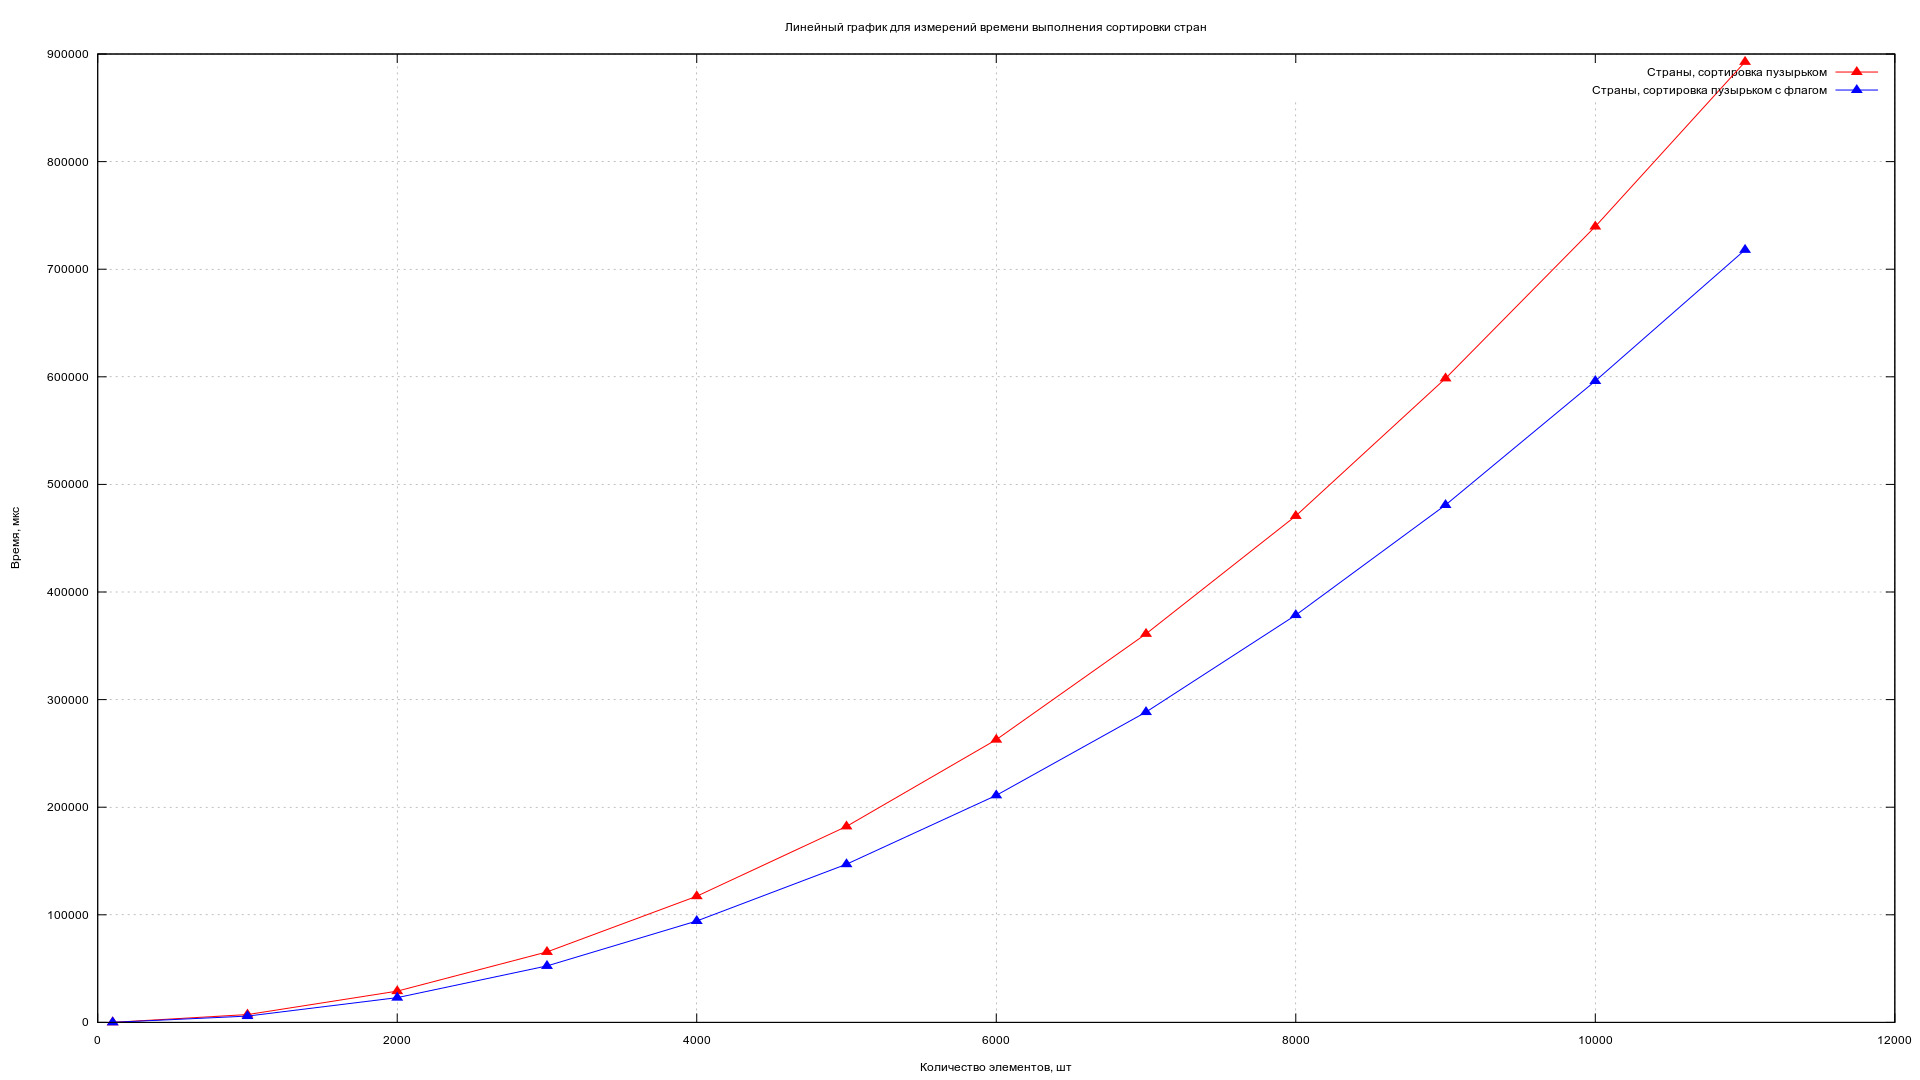
\includegraphics[width=0.88\textwidth]{img/linear_time_together_countries.jpg}
	\captionsetup{font=footnotesize}
	\caption{Зависимость времени между сортировкой стран}
	\label{fig:03}
\end{figure}

\begin{figure}[ht]
	\centering
	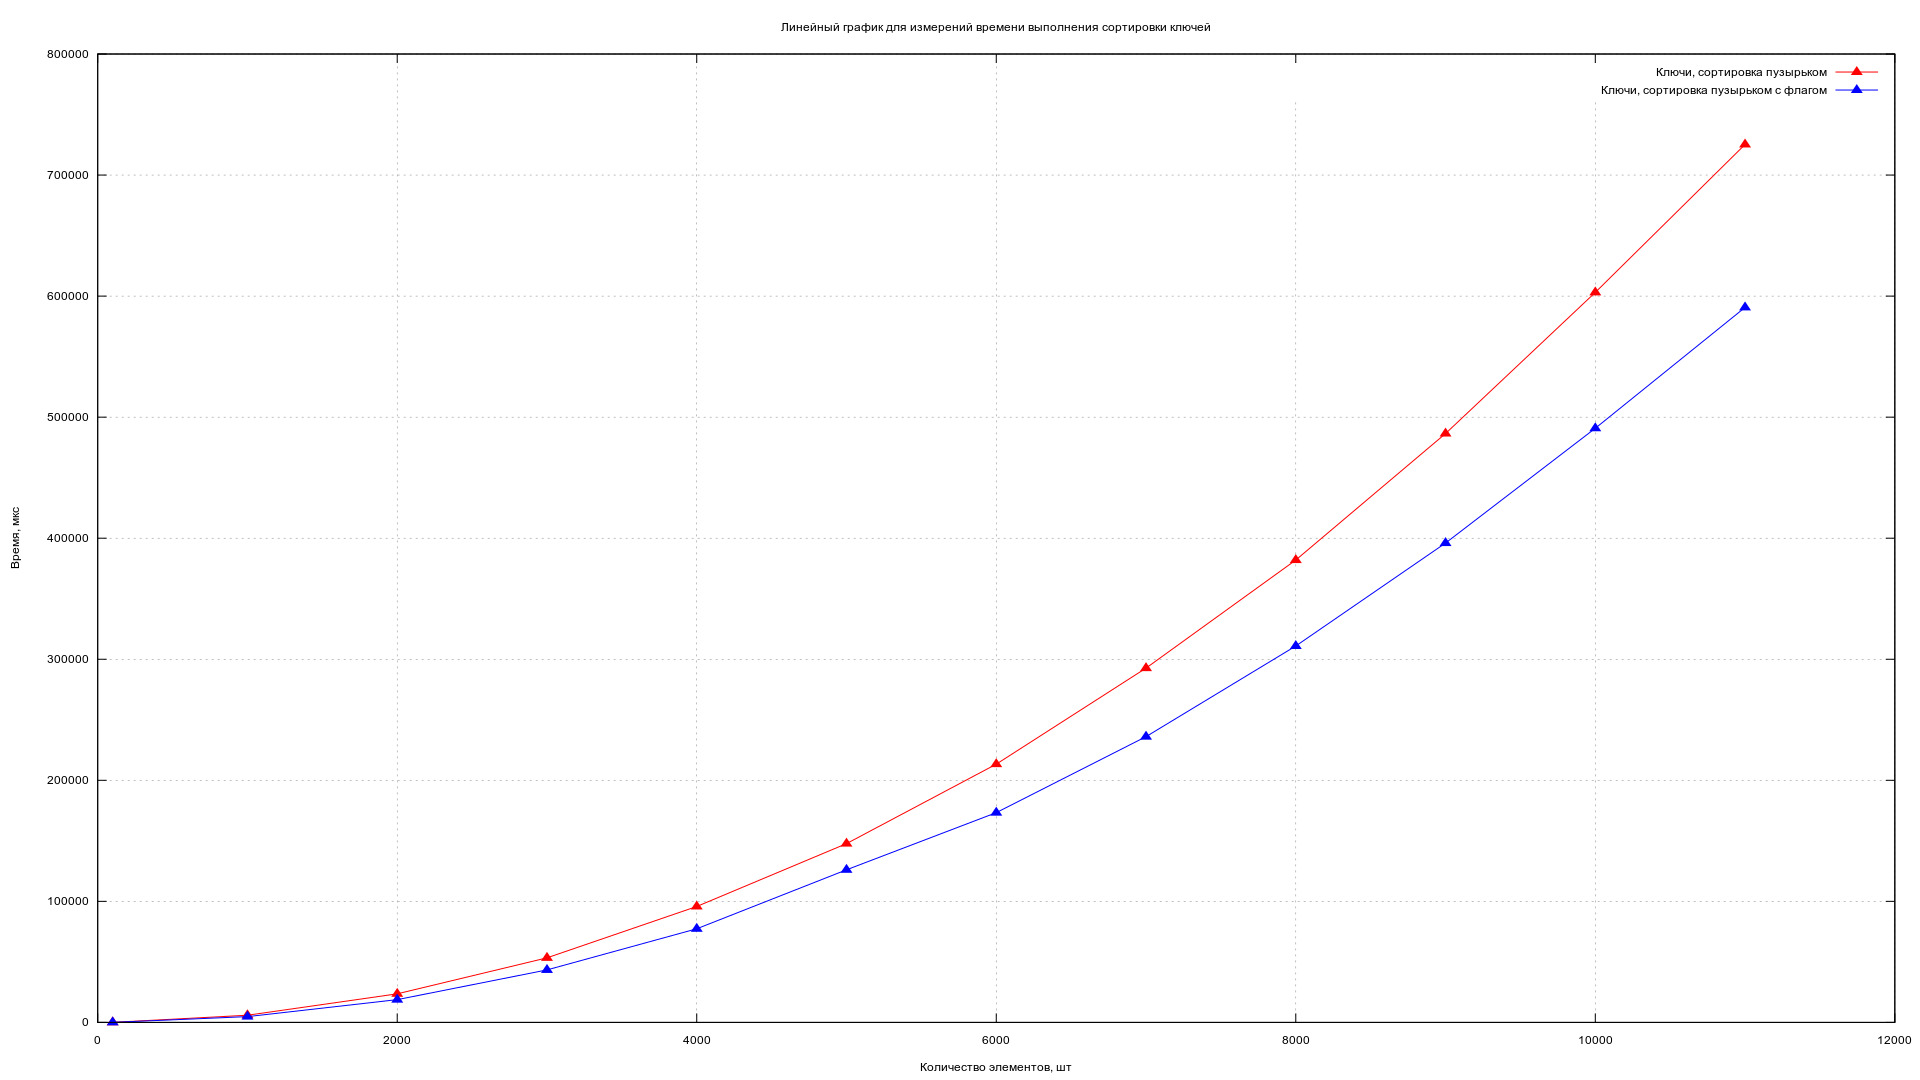
\includegraphics[width=0.88\textwidth]{img/linear_time_together_keys.jpg}
	\captionsetup{font=footnotesize}
	\caption{Зависимость времени между сортировкой ключей}
	\label{fig:04}
\end{figure}